\documentclass[11pt]{article}
\usepackage[a4paper,margin=2.6cm]{geometry}
\usepackage{amsmath,amssymb,amsthm}
\usepackage{booktabs,tabularx,array}
\usepackage{tikz}
\usetikzlibrary{arrows.meta,positioning,calc,patterns.meta}
\usepackage{xcolor}
\usepackage{hyperref}
\usepackage{lineno}
\usepackage{setspace}
\usepackage{enumitem}
\linenumbers
\sloppy
\doublespacing

\newcommand{\lean}[1]{\texttt{#1}}
\newcommand{\Cmax}{C_{\max}}
\definecolor{jobA}{RGB}{120,160,220}
\definecolor{jobB}{RGB}{230,160,90}
\definecolor{jobC}{RGB}{140,200,140}
\definecolor{setup}{RGB}{200,200,200}
\definecolor{robot}{RGB}{200,140,200}

\newtheorem{proposition}{Proposition}
\theoremstyle{definition}
\newtheorem{decision}{Decision}

% A Gantt bar: \bar{row y}{start}{end}{colour}{label}
\newcommand{\gbar}[5]{\fill[#4] (#2,#1-0.35) rectangle (#3,#1+0.35);
  \draw (#2,#1-0.35) rectangle (#3,#1+0.35); \node at ({(#2+#3)/2},#1) {\small #5};}
\newcommand{\gaxis}[2]{\draw[->] (0,#1) -- (#2+0.4,#1);
  \foreach \t in {0,...,#2} \draw (\t,#1+0.08) -- (\t,#1-0.08) node[below] {\scriptsize \t};}

\title{Readings of the Scheduling Zoo's notation in \texttt{schedzoo-lax}\\[2pt]
\large Decisions to sign off before registration}
\author{Working copy for the author}
\date{16 October 2026}

\begin{document}
\maketitle

\begin{abstract}
The formalization turns every problem of The Scheduling Zoo into a Lean
specification. For eight notation values the zoo's text admits more than one
mathematical meaning, and the formalization had to pick one. These choices
are called readings in this document. Registering the submission freezes them, so
each needs a decision. Every section states the zoo's own text, the reading
in Lean, the alternatives, a small instance on which the readings disagree,
what changes formally, and a recommendation. A final section explains how
running time and word size are modelled and proposes fixes for statements
about exact running times. Two findings are errors rather than choices. The
reading of $n=k$ turns 26 result statements into claims about the
unrestricted problem, one of them false unless $\mathrm{P}=\mathrm{NP}$. The
reading of plain serial batching as bounded capacity makes the algorithmic
results of 19 problems claim more than their sources prove.
\end{abstract}

\section{What a reading is, and the decisions at a glance}

A problem of the zoo is a vector of notation values, one per field, such as
$P2|r_j|\sum C_j$. The formalization gives each field a Lean type of values and,
for each value, a condition on instances or schedules. The zoo explains each
value in one sentence of its file \texttt{notation.xml}. Where that sentence
leaves the meaning open, the formalization fixed one. Results of the
literature then become Lean propositions about the problem so defined. A
reading that differs from what the source papers mean makes their results
false or weaker in Lean, even when every proof checks.

Table~\ref{tab:overview} lists the eight readings and the word-size
question. The column ``Changes'' says what moves if the reading is replaced
by the alternative. Edges are the zoo's special-case arrows; ``field-wise''
means the arrow is checked in Lean by comparing the two specifications field
by field, without changing the instance.

\begin{table}[ht]
\centering\small
\renewcommand{\arraystretch}{1.1}
\begin{tabularx}{\textwidth}{>{\raggedright}p{2.5cm}>{\raggedright}p{3.1cm}>{\raggedright}X>{\raggedright\arraybackslash}p{2.7cm}}
\toprule
Notation & Reading in Lean & Changes under the alternative & Recommendation\\
\midrule
$1, P2, \dots, P5$, $n=2,3$ (\S\ref{sec:counts}) & at most $k$ & 40 edges stop being field-wise & keep, but require at least one machine\\
$n=k$ (\S\ref{sec:nk}) & no restriction & 26 result statements & fix: results in the parameter $n$\\
$R$ (\S\ref{sec:R}) & with machine sets & 4 edges stop being field-wise & keep\\
\texttt{s-batch} (\S\ref{sec:batch}) & bounded capacity & 19 problems, 31 relations & fix: unbounded\\
setups (\S\ref{sec:setups}) & may anticipate the job & results of 49 server problems & check sources; make it a value\\
robot (\S\ref{sec:robot}) & no empty moves & results of 23 problems & make empty moves data\\
interval-type orders (\S\ref{sec:orders}) & patterns from a survey & 7 edges & check the original papers\\
$A_m$-orders (\S\ref{sec:orders}) & $m$ of the instance & 1 problem & keep; drop $A_m$ on batching\\
word size (\S\ref{sec:words}) & two conventions & exact running times & one convention for times\\
\bottomrule
\end{tabularx}
\caption{The readings and their status. The section of each row explains the
counts.}
\label{tab:overview}
\end{table}

Throughout, the counts come from the site's \texttt{data/schedulingzoo.json}
(747 problems, 612 edges) and from the Lean files of \texttt{schedzoo-lax} as of
16 October 2026. The small instances were computed by hand and are given
in full, so each can be rechecked.

\section{Number of machines and number of jobs}\label{sec:counts}

\paragraph{The zoo's text.} The value $2$ of the field ``number of machines''
reads ``$m=2$ machines'', and likewise for $3$, $4$, $5$; the value $1$ reads
``Single machine''. The values $n=2$ and $n=3$ of the field ``number of jobs''
read ``The input consists of only 2 jobs'' and ``\dots only 3 jobs''.

\paragraph{The reading in Lean.} The value $k$ means \emph{at most} $k$ machines
(\lean{Counts.lean}, lines 24--51, value \lean{atMost k}, condition $n\le k$).
The same type serves the number of jobs, so $n=2$ and $n=3$ mean at most 2 and
at most 3 jobs. Under this reading $1 \le 2 \le 3 \le 4 \le 5$ is a chain of
special cases checked field by field.

\paragraph{The alternative.} The value $k$ means exactly $k$ machines. Then a
$P2$ instance is not a $P3$ instance. Adding an identical machine changes the
optimum, because jobs may use it. Figure~\ref{fig:p2p3} shows this on three
unit jobs. For uniform machines the extra machine must have a positive speed,
so it can only be made slow, which changes the instance and its encoding. For
unrelated machines a forbidden or very long processing time on the new
machine works, and for shops a machine whose operations all have length $0$
works. Each of these is an encoding that changes the instance, not a
field-wise special case.

\begin{figure}[ht]
\centering
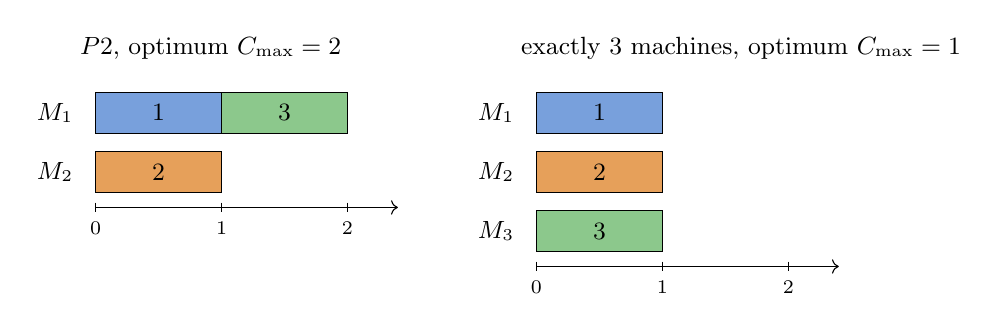
\begin{tikzpicture}[x=1.6cm,y=0.75cm]
\begin{scope}
\node[anchor=west] at (-0.2,3.1) {\small $P2$, optimum $\Cmax=2$};
\node[anchor=east] at (-0.1,2) {\small $M_1$}; \node[anchor=east] at (-0.1,1) {\small $M_2$};
\gbar{2}{0}{1}{jobA}{1} \gbar{2}{1}{2}{jobC}{3} \gbar{1}{0}{1}{jobB}{2}
\gaxis{0.4}{2}
\end{scope}
\begin{scope}[xshift=5.6cm]
\node[anchor=west] at (-0.2,3.1) {\small exactly $3$ machines, optimum $\Cmax=1$};
\node[anchor=east] at (-0.1,2) {\small $M_1$}; \node[anchor=east] at (-0.1,1) {\small $M_2$};
\node[anchor=east] at (-0.1,0) {\small $M_3$};
\gbar{2}{0}{1}{jobA}{1} \gbar{1}{0}{1}{jobB}{2} \gbar{0}{0}{1}{jobC}{3}
\gaxis{-0.6}{2}
\end{scope}
\end{tikzpicture}
\caption{Three unit jobs, objective $\Cmax$. An extra identical machine
lowers the optimum from 2 to 1, so ``exactly 2 machines'' is not a special
case of ``exactly 3 machines''.}
\label{fig:p2p3}
\end{figure}

\paragraph{What changes.} Of the 89 edges that change the number of
machines, 49 go from ``any number'' to a value $k$. They are field-wise under both
readings. The other 40 go from a larger to a smaller value, such as $P2 \to 1$ or
$F3 \to F2$. Under ``exactly'' they stop being field-wise. Of these, 13 are on
parallel machines and 27 on shops. No edge between job counts changes, because the
data has no edge from $n=3$ to $n=2$. The zoo itself guards its rules
$1 \to 2 \to \dots \to 5$ by ``not processing times; not preemption''. That
guard makes sense only under ``exactly'', where a padding with dummy jobs or
machines would break $p_j=1$ or preemption. Under ``at most'' the guard is
unnecessary.

\paragraph{What the results mean.} A hardness result for exactly $k$
machines remains true for at most $k$, since the latter has more instances.
An algorithm for exactly $k$ machines becomes, in Lean, a claim for every
$m\le k$. The smaller cases are usually classical problems that the same
source or an older one solves, so this is a small strengthening of the source.
We have not checked this source by source; the review of the algorithmic
results with a fixed number of machines should include it.

\paragraph{A side effect.} The value $1$ also admits instances with
\emph{no} machine. The proof \lean{EncodingsFlow} handles this case
separately (with no machine the answer is known and moves into the threshold).
\lean{PLAN.md}, decision~3, says the opposite, that a single machine is
identical machines with exactly one machine.

\begin{decision}
Keep ``at most $k$'' for machines and jobs, but require at least one
machine (the value $k$ means $1 \le m \le k$). Correct \lean{PLAN.md}. The 40
downward edges stay field-wise, and instances without machines disappear,
so \lean{EncodingsFlow} loses its special case.
\end{decision}

\section{The value \texorpdfstring{$n=k$}{n=k}}\label{sec:nk}

\paragraph{The zoo's text.} ``The input consists of only $k$ jobs.''

\paragraph{The reading in Lean.} The value is a marker with no condition
(\lean{Counts.lean}, lines 13--14 and 44, value \lean{constant}). The instances
of $J2|n=k|\sum w_jU_j$ are therefore all instances of $J2||\sum w_jU_j$.

\paragraph{Why this is an error.} The results the zoo records for these
problems are statements \emph{for every fixed number of jobs}, such as
``polynomial when the number of jobs is a constant''. Lean states them as
\lean{InP} of the problem, which under the marker reading means polynomial for
all $n$. There are 26 such statements, 22 in \lean{ZooShopsResults} and 4 in
\lean{ZooPreemptiveShopsResults}; 15 of them are \lean{InP}. One is false
unless $\mathrm{P}=\mathrm{NP}$.

\begin{proposition}
If $\mathrm{P}\ne\mathrm{NP}$, then $J2||\sum w_jU_j$ is not in P, so the
statement \lean{ZooShopsResults.p92\_r0}, which reads \lean{InP (R.at p92)} for
$J2|n=k|\sum w_jU_j$, is false under the marker reading.
\end{proposition}

\begin{proof}
$1||\sum w_jU_j$ is NP-hard (Karp). Given an instance of it, make every job a
job of the job shop with one operation on machine 1. A schedule of the shop is
a schedule of the single machine with the same late jobs, and conversely.
Under the marker reading this instance, with any number of jobs, is an
instance of $J2|n=k|\sum w_jU_j$.
\end{proof}

A second statement is attached to the wrong parameter.
\lean{ZooPreemptiveShopsResults.p0\_r0} states $J|n=k;pmtn|\Cmax$ as
pseudo-polynomial for every fixed \emph{number of machines}, while the source
(Brucker, Kravchenko and Sotskov 1999) is titled ``\dots with a fixed number
of jobs''. The zoo's data tags the result with $m$, and the generator copied the
tag.

\paragraph{The alternatives.} (i) $n=k$ means at most $k$ jobs for one
fixed $k$. Then the problem is a family indexed by $k$, which no single
specification expresses. (ii) The node keeps all instances, and its results are
read in the parameter $n$. Then ``polynomial for constant $n$'' becomes
\lean{InPFixed} in \lean{Ops.n}, and ``pseudo-polynomial for constant $n$''
becomes \lean{PseudoPolyFixed} in \lean{Ops.n}. The 14 edges into $n=2$ and
$n=3$ remain field-wise under both.

\begin{decision}
Take (ii). Keep the marker, and have \lean{tools/results.py} translate every
result of an $n=k$ problem in the parameter $n$, or in $n$ together with the
parameter the data names. Review the 26 statements one by one against their
sources, starting with the 15 \lean{InP} ones and \lean{p0\_r0} above.
\end{decision}

\section{Unrelated machines with machine sets}\label{sec:R}

\paragraph{The zoo's text.} $R$: ``Processing time of job $j$ on machine $i$
is some given length $p_{ij}$.'' $M_j$: ``Every job $j$ needs to be scheduled on
one machine out of a given set $M_j$.'' The zoo's own rule $M_j;R \to R$
(added upstream by Dürr in 2023) says ``processing times $p_{ij}=\infty$ can be
used to encode $M_j$''.

\paragraph{The reading in Lean.} Every $R$ problem carries the machine-set
field with value \lean{sets} (\lean{coverage.py}, lines 130--138). An $R$
instance may thus forbid a machine for a job, which stands for $p_{ij}=\infty$.
Then $P|M_j$ and $Q|M_j$ are field-wise special cases of $R$.

\paragraph{The alternative.} $p_{ij}$ is finite. Then a forbidden machine
must be encoded by a large processing time, larger than any schedule worth
considering, such as $\sum_j \max_i p_{ij}+1$. That changes the instance and
its size, and whether it keeps the answer depends on the objective. Four
edges would stop being field-wise, all four added by the site's
eligibility rule: $R||\Cmax\to P|M_j|\Cmax$, $R||\sum C_j \to Q|M_j|\sum C_j$,
$R||\sum w_jC_j\to P|M_j|\sum w_jC_j$ and $R||\sum w_jZ_j \to P|M_j|\sum w_jZ_j$.

\paragraph{A point to check.} Parameters that read the matrix $(p_{ij})$, namely
$p_{\max}$, its rank and the number of kinds of machines, must ignore the
forbidden entries. In Lean they are computed from the finite times, and a
forbidden pair is a separate datum, so this holds by construction. A result
for $R$ with one of these parameters whose source assumes finite times must
still be checked to cover forbidden pairs.

\begin{decision}
Keep the reading. It is the zoo's own (Dürr's rule), and the standard
convention in the literature on unrelated machines.
\end{decision}

\section{Serial batching and its capacity}\label{sec:batch}

\paragraph{The zoo's text.} \texttt{s-batch}: ``Serial batching. The jobs have
to be processed in batches. The processing time of a batch is the total
processing time over all jobs in the batch. If a new batch is started, a
constant setup time $s$ occurs.'' \texttt{s-batch($\infty$)} adds ``There is no
limit on the number of jobs in a batch'', and \texttt{s-batch(b)} says ``A
batch consists of maximal $b$ jobs''. The zoo has the rules
$\texttt{s-batch}(\infty)\to\texttt{s-batch}$ and
$\texttt{s-batch}(\infty)\to\texttt{s-batch(b)}$, and none between
\texttt{s-batch} and \texttt{s-batch(b)}.

\paragraph{The reading in Lean.} Plain \texttt{s-batch} is bounded capacity,
with the bound $b$ part of the instance (\lean{coverage.py}, lines 178--184).
So $1|\texttt{s-batch}|\sum w_jU_j$ and $1|\texttt{s-batch(b)}|\sum w_jU_j$ are the
same Lean specification, and unbounded capacity is the special case $b=n$.

\paragraph{The alternative.} In Brucker's book and in the classical papers on
serial batching, plain \texttt{s-batch} means unbounded capacity, and a bound
is written separately. Under that reading \texttt{s-batch} and
\texttt{s-batch($\infty$)} are the same problem and \texttt{s-batch(b)}
generalizes both. Figure~\ref{fig:sbatch} shows an instance on which a
capacity bound matters.

\begin{figure}[ht]
\centering
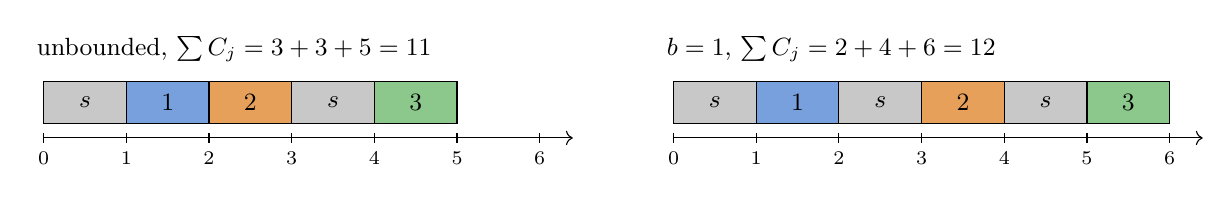
\begin{tikzpicture}[x=1.05cm,y=0.75cm]
\begin{scope}
\node[anchor=west] at (-0.2,1.9) {\small unbounded, $\sum C_j=3+3+5=11$};
\gbar{1}{0}{1}{setup}{$s$} \gbar{1}{1}{2}{jobA}{1} \gbar{1}{2}{3}{jobB}{2}
\gbar{1}{3}{4}{setup}{$s$} \gbar{1}{4}{5}{jobC}{3}
\gaxis{0.4}{6}
\end{scope}
\begin{scope}[xshift=8.0cm]
\node[anchor=west] at (-0.2,1.9) {\small $b=1$, $\sum C_j=2+4+6=12$};
\gbar{1}{0}{1}{setup}{$s$} \gbar{1}{1}{2}{jobA}{1}
\gbar{1}{2}{3}{setup}{$s$} \gbar{1}{3}{4}{jobB}{2}
\gbar{1}{4}{5}{setup}{$s$} \gbar{1}{5}{6}{jobC}{3}
\gaxis{0.4}{6}
\end{scope}
\end{tikzpicture}
\caption{Serial batching on one machine, setup $s=1$, three unit jobs,
objective $\sum C_j$. Every job of a batch completes with its batch. Without a
bound the best batching is $\{1,2\},\{3\}$ with $\sum C_j=11$; one batch gives
12. With at most one job per batch the only schedule gives 12.}
\label{fig:sbatch}
\end{figure}

\paragraph{What changes.} The zoo has 19 problems with plain \texttt{s-batch}.
Under the Lean reading each contains every bounded instance. A hardness result
proved for unbounded capacity remains true, since unbounded capacity is the
case $b=n$. An algorithm proved for unbounded capacity does not cover bounded
capacity, so the Lean statements of the algorithmic results claim more than
their sources prove. This affects, among others, $1|\texttt{s-batch}|\sum C_j$,
$1|\texttt{s-batch}|\sum U_j$ and $1|\texttt{s-batch}|\sum w_jU_j$
(pseudo-polynomial), $1|\texttt{s-batch};prec|L_{\max}$ and the cases with
$p_j=p$. The 31 relations of \lean{BatchingZeroSetup}, which read a
single machine as batching with setup $0$ and capacity $1$, use the bounded
reading. Under the unbounded reading they need a different argument. With
setup $0$, splitting a batch into single jobs in the same order never delays
a job, so for a regular objective the optimum is attained by batches of one
job.

\begin{decision}
Read \texttt{s-batch} as \texttt{s-batch($\infty$)}, change the mapping in
\lean{coverage.py}, regenerate \lean{ZooSerialBatching}, and reprove
\lean{BatchingZeroSetup} for the serial case with the splitting argument above.
For parallel batching the zoo's text of \texttt{p-batch} does say ``maximal
$b$ jobs'', so it stays bounded.
\end{decision}

\section{Setup times}\label{sec:setups}

\paragraph{The zoo's text.} The single server: ``A single server is loading the
job $J_j$ or operation $O_{ij}$ on the machine which requires a setup time.
These setup periods cannot overlap.'' The values $s_j=s$, $s_j=1$, $s_{ij}=s$
and $s_{ij}=1$ only fix the lengths. Batch setups (a value this site adds,
for open problem 14 of Mnich and van Bevern) read ``a setup time $s_{pq}$
occurs when the machine switches from a job of batch $p$ to a job of batch
$q$''.

\paragraph{The reading in Lean.} The setup of a job or operation ends exactly
when its processing starts (\lean{Servers.lean}, lines 10--19 and 72--78). During
the setup the machine and the server are busy. For serial batching a batch
starts no earlier than $s$ after the previous batch, and the first one no
earlier than $s$. Batch setups are required between \emph{every} two operations
of different batches on a machine, not only between consecutive ones
(\lean{Operations.lean}, lines 408--418).

\paragraph{Three questions hide in this reading.}
\begin{enumerate}[leftmargin=*]
\item \emph{May there be a gap between setup and processing?} For the
objectives of the zoo this does not matter. Every objective is regular
(non-decreasing in the completion times), and moving the processing left to
the end of its setup keeps every constraint.
\item \emph{May a setup anticipate the job?} In Lean the setup of a job may
run before its release date, and in a shop the setup of an operation may
overlap the job's previous operation on another machine. The word
``loading'' suggests the job must be present, which is the usual
non-anticipatory model. Figure~\ref{fig:setup} shows that the readings differ.
\item \emph{Between which batches is a batch setup charged?} Lean charges
it between every pair of operations of different batches on a machine. The
usual model charges only consecutive ones. They differ when the setup times
violate the triangle inequality.
\end{enumerate}

\begin{figure}[ht]
\centering
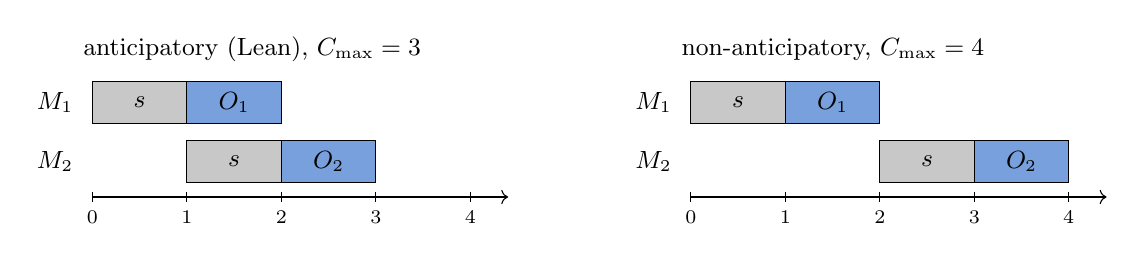
\begin{tikzpicture}[x=1.2cm,y=0.75cm]
\begin{scope}
\node[anchor=west] at (-0.2,2.9) {\small anticipatory (Lean), $\Cmax=3$};
\node[anchor=east] at (-0.1,2) {\small $M_1$}; \node[anchor=east] at (-0.1,1) {\small $M_2$};
\gbar{2}{0}{1}{setup}{$s$} \gbar{2}{1}{2}{jobA}{$O_1$}
\gbar{1}{1}{2}{setup}{$s$} \gbar{1}{2}{3}{jobA}{$O_2$}
\gaxis{0.4}{4}
\end{scope}
\begin{scope}[xshift=7.6cm]
\node[anchor=west] at (-0.2,2.9) {\small non-anticipatory, $\Cmax=4$};
\node[anchor=east] at (-0.1,2) {\small $M_1$}; \node[anchor=east] at (-0.1,1) {\small $M_2$};
\gbar{2}{0}{1}{setup}{$s$} \gbar{2}{1}{2}{jobA}{$O_1$}
\gbar{1}{2}{3}{setup}{$s$} \gbar{1}{3}{4}{jobA}{$O_2$}
\gaxis{0.4}{4}
\end{scope}
\end{tikzpicture}
\caption{$F2;S1$ with one job, unit operations and unit setups, objective
$\Cmax$. In Lean the server may set up $M_2$ while the job is still on $M_1$.
If the job must be on the machine for its setup, the setup of $M_2$ waits.}
\label{fig:setup}
\end{figure}

Two more instances, computed the same way. Serial batching, one job with
$p=1$ and release date $5$, setup $s=2$. In Lean the setup runs during
$[3,5]$ and $C=6$; if the setup may start only once the job is released,
$C=8$. Batch setups on one machine, three unit jobs in batches $1,2,3$, with
$s_{12}=s_{23}=0$, $s_{13}=5$ and every other $s_{pq}=10$. In Lean the order
$1,2,3$ needs $S_3 \ge C_1 + s_{13} = 6$, so $\Cmax = 7$, and no other order is
better. Charging only consecutive pairs gives $\Cmax = 3$.

\paragraph{What changes.} The zoo has 49 problems with a single server and one
with batch setups. The edges between them are field-wise under every
reading, since the field order does not change. What changes is the meaning of
their results. For a result whose source uses non-anticipatory setups, an
algorithm stated in Lean claims to solve a problem with more freedom, and a
hardness result may not transfer.

\begin{decision}
Do not choose one reading for all problems. Make anticipation a value of the
setup field (anticipatory, non-anticipatory), check the model of each source,
and give each problem the value its source uses. For batch setups, charge only
consecutive pairs, which is the standard model; for the one problem that uses
them, check the source of open problem 14.
\end{decision}

\section{The transport robot}\label{sec:robot}

\paragraph{The zoo's text.} ``We are given a single robot that can transport
the operations of a job from one machine to another. The robot can make at
most one transportation per time.''

\paragraph{The reading in Lean.} Every transport starts no earlier than the
completion of the operation, lasts for its delay, ends no later than the start of
the next operation, and no two transports overlap (\lean{Transportation.lean},
lines 30--35 and 93--100). The robot has no position, so it needs no time to
travel empty to the next pickup.

\paragraph{The alternative.} The model of Hurink and Knust, cited for these
problems, has empty moving times $t'_{kl}$. This is the time the robot needs to get
from machine $k$, where it dropped a job, to machine $l$, where it picks up the
next one. Whether a given paper sets them to zero must be checked in the paper.
Figure~\ref{fig:robot} shows that they matter.

\begin{figure}[ht]
\centering
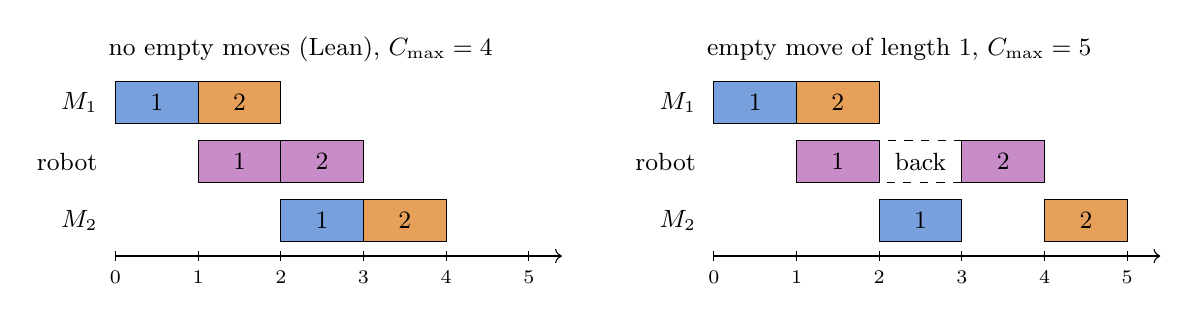
\begin{tikzpicture}[x=1.05cm,y=0.75cm]
\begin{scope}
\node[anchor=west] at (-0.2,3.9) {\small no empty moves (Lean), $\Cmax=4$};
\node[anchor=east] at (-0.1,3) {\small $M_1$}; \node[anchor=east] at (-0.1,2) {\small robot};
\node[anchor=east] at (-0.1,1) {\small $M_2$};
\gbar{3}{0}{1}{jobA}{1} \gbar{3}{1}{2}{jobB}{2}
\gbar{2}{1}{2}{robot}{1} \gbar{2}{2}{3}{robot}{2}
\gbar{1}{2}{3}{jobA}{1} \gbar{1}{3}{4}{jobB}{2}
\gaxis{0.4}{5}
\end{scope}
\begin{scope}[xshift=7.6cm]
\node[anchor=west] at (-0.2,3.9) {\small empty move of length 1, $\Cmax=5$};
\node[anchor=east] at (-0.1,3) {\small $M_1$}; \node[anchor=east] at (-0.1,2) {\small robot};
\node[anchor=east] at (-0.1,1) {\small $M_2$};
\gbar{3}{0}{1}{jobA}{1} \gbar{3}{1}{2}{jobB}{2}
\gbar{2}{1}{2}{robot}{1} \draw[dashed] (2,2-0.35) rectangle (3,2+0.35); \node at (2.5,2) {\small back}; \gbar{2}{3}{4}{robot}{2}
\gbar{1}{2}{3}{jobA}{1} \gbar{1}{4}{5}{jobB}{2}
\gaxis{0.4}{5}
\end{scope}
\end{tikzpicture}
\caption{$F2;R1$, two jobs with unit operations and unit transport times,
objective $\Cmax$. With an empty move of length 1 from $M_2$ back to $M_1$, the
second transport starts at 3 and the optimum rises from 4 to 5.}
\label{fig:robot}
\end{figure}

\paragraph{What changes.} The zoo has 23 problems with a robot, all flow
shops. The 8 edges that touch them only compare shapes and survive. The
results would change meaning, as for setups.

\begin{decision}
Add empty moving times as data of the robot, with the present reading as the
special case where they are all zero. Then both readings are specifications,
the present one is a field-wise special case of the other, and each result is
attached to the reading of its source.
\end{decision}

\section{Interval-type orders and \texorpdfstring{$A_m$}{A\_m}-orders}\label{sec:orders}

\paragraph{The zoo's text.} The zoo cites the papers that define
quasi-interval orders (Moukrim 1999), over-interval orders (Chardon and
Moukrim 2005) and $A_m$-orders (Moukrim and Quilliot 1997) and gives no
definition. Its rules make interval $\subseteq$ quasi-interval $\subseteq$
over-interval $\subseteq A_m$ $\subseteq$ arbitrary orders.

\paragraph{The reading in Lean.} The definitions come from the survey of Prot
and Bellenguez-Morineau (arXiv:1510.04833), Figures 8 and 9 and Definition 7
(\lean{Precedence.lean}, lines 38--47 and 152--176). An order is
\emph{over-interval} if it contains neither the pattern of
Figure~\ref{fig:patterns}(a) nor its reverse (b) as an induced suborder on five
jobs, and \emph{quasi-interval} if moreover it does not contain (c).
Interval orders contain none of the three, which is proved in Lean
(\lean{quasi\_of\_interval}).

\begin{figure}[ht]
\centering
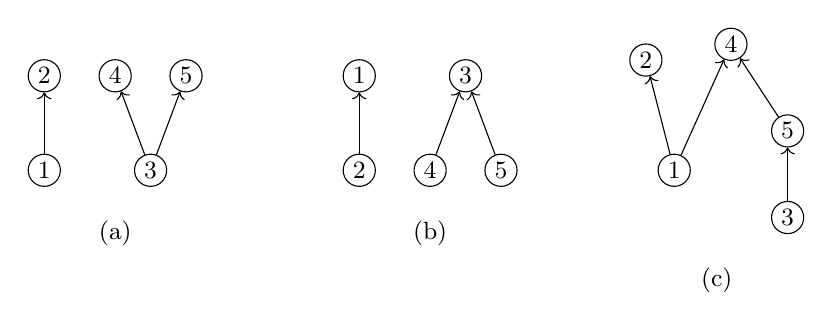
\begin{tikzpicture}[every node/.style={circle,draw,inner sep=1.5pt,font=\small},x=0.9cm,y=1cm]
\begin{scope}
\node (a1) at (0,0) {1}; \node (a2) at (0,1.2) {2};
\node (a3) at (1.5,0) {3}; \node (a4) at (1,1.2) {4}; \node (a5) at (2,1.2) {5};
\draw[->] (a1)--(a2); \draw[->] (a3)--(a4); \draw[->] (a3)--(a5);
\node[draw=none] at (1,-0.8) {(a)};
\end{scope}
\begin{scope}[xshift=4cm]
\node (b2) at (0,0) {2}; \node (b1) at (0,1.2) {1};
\node (b4) at (1,0) {4}; \node (b5) at (2,0) {5}; \node (b3) at (1.5,1.2) {3};
\draw[->] (b2)--(b1); \draw[->] (b4)--(b3); \draw[->] (b5)--(b3);
\node[draw=none] at (1,-0.8) {(b)};
\end{scope}
\begin{scope}[xshift=8cm]
\node (c1) at (0,0) {1}; \node (c3) at (1.6,-0.6) {3};
\node (c2) at (-0.4,1.4) {2}; \node (c5) at (1.6,0.5) {5}; \node (c4) at (0.8,1.6) {4};
\draw[->] (c1)--(c2); \draw[->] (c1)--(c4); \draw[->] (c3)--(c5); \draw[->] (c5)--(c4);
\node[draw=none] at (0.6,-1.4) {(c)};
\end{scope}
\end{tikzpicture}
\caption{The three forbidden patterns, as Hasse diagrams (an arrow
$i\to j$ means $i\prec j$; in (c) also $3\prec 4$ by transitivity). An order
contains a pattern if five of its jobs are related exactly as drawn. Over-interval
orders avoid (a) and (b); quasi-interval orders avoid all three.}
\label{fig:patterns}
\end{figure}

$A_m$-orders depend on a number $m$. In Lean $m$ is the number of machines of
the instance, and $1$ for batching. The order is an $A_m$-order if for any two
sets $A,B$ of at most $m$ pairwise unrelated jobs, at most $m$ jobs of
$A\cup B$ lie in $A\cap B$ or have a predecessor in $A\cup B$, and likewise
with successors. The survey's Definition 7 writes $A\cup V$ where $A\cup B$ is
meant; Lean reads $A\cup B$ (\lean{UPSTREAM.md}).

\begin{proposition}
Under this definition every order is an $A_1$-order and an $A_2$-order.
\end{proposition}

\begin{proof}
The condition reads only the order induced on $A\cup B$, which has at most
$2m$ jobs. For $m\le 2$ it therefore suffices to check every order on at most
four jobs with every choice of $A$ and $B$. We checked every order on at most
five jobs by computer (4231 orders on five jobs), and none fails for
$m=1,2,3$. The smallest order that is not an $A_3$-order has six jobs:
$a\prec c$, $a\prec d$, $b\prec e$, $b\prec f$, with $A=\{b,c,d\}$ and
$B=\{a,e,f\}$. Four jobs of $A\cup B$ have a predecessor in it.
\end{proof}

So on batching, where Lean sets $m=1$, the class $A_m$ imposes nothing. On
two machines this matches what is known, since two-machine scheduling of unit
jobs is polynomial for every order (Coffman and Graham).

\paragraph{What changes.} Three zoo problems use these classes, one each:
$P|\text{quasi-interval};p_j=p|\Cmax$, $P|\text{over-interval};p_j=p|\Cmax$ and
$P|pmtn;A_m\text{-order}|\Cmax$. Seven edges involve them. The inclusion
over-interval $\subseteq A_m$ is not in Lean yet; no edge of the data needs it.

\begin{decision}
Check Figures 8 and 9 of the survey against the original definitions of
Moukrim (1999) and Chardon and Moukrim (2005), and Definition 7 against
Moukrim and Quilliot (1997). Keep $m$ as the instance's number of machines,
which matches the title of the one source (``on a fixed number of identical
parallel machines''). Remove the $A_m$ value from the batching family, where it
says nothing.
\end{decision}

\section{Running time and word size}\label{sec:words}

This section explains how Lean measures running time, because a decision about
fine-grained results depends on it. The machine is the word RAM of the
registered submission lax-808846.

\paragraph{The machine.} A program is a list of instructions on
memory cells that hold $\ell$-bit words. The instructions are load and store
through an address cell, addition, truncated subtraction, multiplication,
division, bitwise and, left shift, bitwise not, jumps, and reading the input.
Each costs one step. Every result is reduced modulo $2^\ell$. The word length
$\ell$ is not an instruction's argument; it is fixed for a run. The input is a
list of natural numbers, read through an index. There is no randomness and no
space measure.

\paragraph{The question of word size.} The cost of an algorithm depends on
how large $\ell$ may be. With words of $\ell$ bits a single instruction does
$\ell$ bit operations at once. If $\ell$ may grow with the running time,
algorithms can pack a whole dynamic-programming table into one word. If $\ell$ is
$O(\log)$ of the input, as in the standard word RAM, a word holds one number of
the input and no more.

\paragraph{Two conventions in the formalization.} Figure~\ref{fig:words} shows
which notions use which convention.
\begin{enumerate}[leftmargin=*]
\item \emph{Short words.} The exact running times \lean{DecidesWithin} and
\lean{DecidesExact}, the timed approximations, and \lean{ETH} require the
program to work at every word length $\ell$ with
$(|u|+M+2)^c\le 2^\ell$, where $|u|$ is the number of entries of the input,
$M$ its largest number and $c$ the program's constant. So
$\ell\ge c\log_2(|u|+M+2)$. Since the program must also work at the smallest
such $\ell$, it cannot profit from longer words. This is the standard
convention $w = \Theta(\log(n+M))$ of Fredman--Willard and Hagerup.
\item \emph{Long words.} The classes P, pseudo-polynomial, XP, FPT, the
approximation classes and kernels go through the registered notions of
lax-496464. There, a single bound $B$ is both the time bound and the least word
length. So a polynomial-time algorithm may use words of polynomially many bits,
and a pseudo-polynomial one words of pseudo-polynomially many bits.
\end{enumerate}

\begin{figure}[ht]
\centering
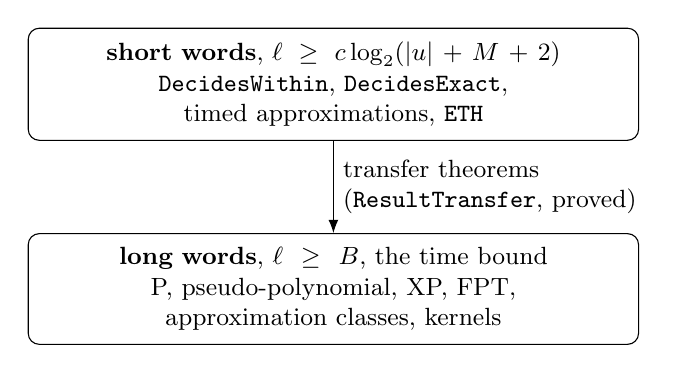
\begin{tikzpicture}[box/.style={draw,rounded corners,align=center,font=\small,inner sep=5pt,text width=7.4cm}]
\node[box] (short) at (0,0) {\textbf{short words}, $\ell \ge c\log_2(|u|+M+2)$\\
\lean{DecidesWithin}, \lean{DecidesExact}, timed approximations, \lean{ETH}};
\node[box] (long) at (0,-2.6) {\textbf{long words}, $\ell \ge B$, the time bound\\
P, pseudo-polynomial, XP, FPT, approximation classes, kernels};
\draw[-{Latex}] (short.south) -- node[right,font=\small,align=left] {transfer theorems\\ (\lean{ResultTransfer}, proved)} (long.north);
\end{tikzpicture}
\caption{The two word-size conventions. A running time proved with short words gives
the class with long words. The converse direction is neither available nor
wanted.}
\label{fig:words}
\end{figure}

\paragraph{Why long words are harmless for classes.} A Turing machine
simulates one instruction on $B$-bit words in time polynomial in $B$. So a
problem decided in polynomial time with polynomially long words is in P in
every model, and similarly for pseudo-polynomial time, XP and FPT. This is why
the registered notions could choose long words. They are needed, because the
registered NP-hardness and W-hardness are stated with them, and our hardness
results compose with theirs.

\paragraph{Why long words are harmful for running times.} With
pseudo-polynomially long words, the subset-sum table
$S \leftarrow S \lor (S \ll a_i)$ costs a shift and a bitwise or, a constant
number of instructions per item. So subset sum
takes $O(n)$ instructions inside \lean{PseudoPoly}. A pseudo-polynomial
algorithm in this sense says nothing about the degree of its polynomial, and
the same holds for every class with long words. For classes this is fine; for
fine-grained statements it is not.

\paragraph{Further points about exact running times.}
\begin{enumerate}[leftmargin=*]
\item \emph{Reading the input is free in the bound.} \lean{DecidesWithin}
bounds the steps by $c\,(T(x)+1)$ with no term for the input length, and an
indexed read costs one step. So a sublinear $T$ is meaningful. A lower bound
$\lnot\,$\lean{DecidesWithin}$\,T$ for a $T$ below the input length can then be
true for the trivial reason that the input cannot be read.
\item \emph{Large numbers widen the words.} The word length grows with the
largest number $M$ of the instance, threshold included. A reduction that
produces numbers of $\Theta(n)$ bits gives the scheduling algorithm words of
$\Theta(n)$ bits with unit-cost multiplication. For ETH lower bounds of the
form $2^{o(n)}$ this is absorbed. For polynomial lower bounds it is not,
unless the reduction keeps the numbers polynomial.
\item \emph{Composition of reductions.} The registered equivalence between
the word RAM and Turing machines has an unspecified polynomial overhead. So a
reduction stated by a Turing machine, like \lean{NPHardIn}, cannot carry
exponents. Fine-grained reductions must be word-RAM programs composed with
the cost library (\lean{Cost.compose\_solves}, which gives the exact cost of
the composition).
\item \emph{The instruction set.} Exact counts in \lean{DecidesExact} depend on
it. For example, bitwise or costs three instructions. This is a property of
the registered machine and is fine, but a constant-free running time is a
claim about this machine, not about every word RAM.
\end{enumerate}

\paragraph{Proposed fixes.}
\begin{enumerate}[leftmargin=*]
\item \emph{One convention for every running time.} Every statement that names
a running time, upper or lower, uses short words. Classes keep long words, and
are reached from running times only through the transfer theorems. This is
already how algorithms enter (an uploaded algorithm proves
\lean{DecidesWithin}), so the fix is a rule plus a check in
\lean{tools/results.py} that no statement mixes the two.
\item \emph{Lower bounds include the input.} State every conditional lower
bound for $T(x)+|u|$, so that it cannot hold for the trivial reason above.
\item \emph{Fine-grained hypotheses with short words.} Define SETH, OV, 3SUM,
APSP, $k$-Clique and Min-Plus Convolution in the style of \lean{ETH}, on short
words, each for an explicit problem on words. For problems with numbers, state
the hypothesis for numbers polynomial in the input length, which is how
these conjectures are stated in the literature.
\item \emph{Reductions keep numbers small or say so.} A fine-grained reduction
in Lean is a word-RAM program with an exact cost and a bound on the numbers
it writes, so the word length on the target side is known.
\end{enumerate}

\begin{decision}
Adopt the four fixes. Only the first touches existing statements, and only as a
check; the others are additions.
\end{decision}

\section*{What is verified in this document}

Every count of problems and edges was computed from the site's data and the
Lean files on 16 October 2026. The statements \lean{p92\_r0} and
\lean{p0\_r0} were read in the Lean files. The instances of the figures were
computed by hand and can be rechecked from the captions. The $A_m$ proposition
was checked by computer for all orders on at most five jobs. The descriptions
of Brucker's convention for serial batching, of the Hurink--Knust robot model
and of the original definitions of the interval-type orders are from memory or
from the survey, not from the original papers, and are marked as things to
check in the decisions.

\end{document}
